\begin{sectionblock}{Focus}
  The project focuses on \textbf{linear algebra} as a course which can
  be taught from a variety of perspectives.  Some students seek
  real-world applications, and others want to see the theory developed
  in an abstract setting.

\end{sectionblock}

\begin{sectionblock}{Platform}
%  \begin{columns}
%    \begin{column}{0.5\textwidth}
%      The project team developed a platform for hosting and disseminating
%%      open mathematics content.
%    \end{column}
%    \begin{column}{0.5\textwidth}
%        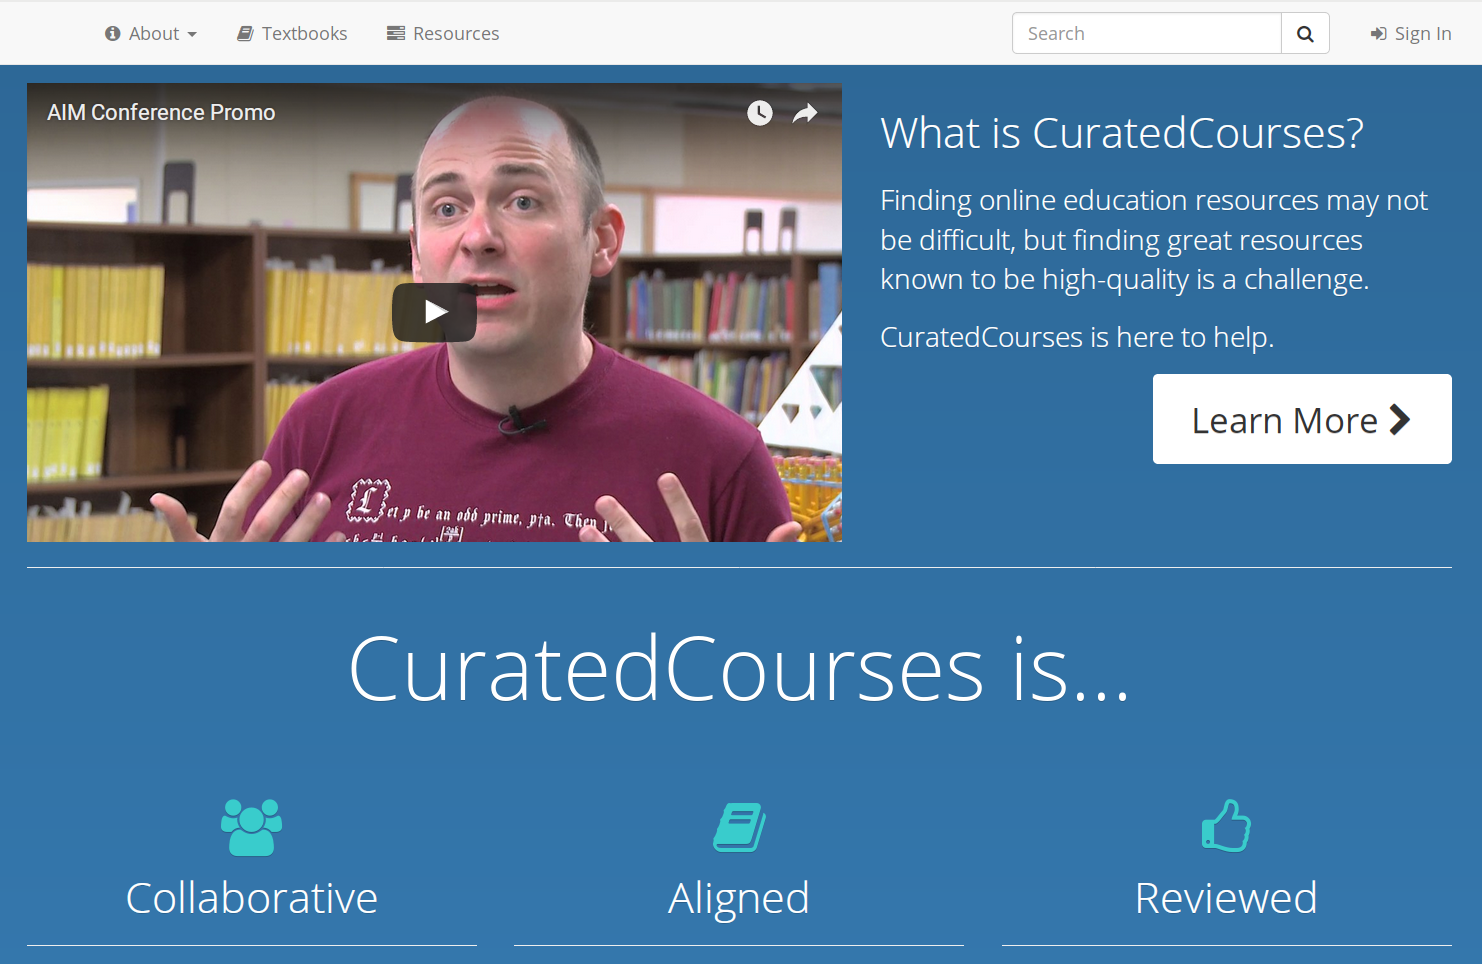
\includegraphics[width=\textwidth]{landing-page.png}
%    \end{column}
%  \end{columns}

  \begin{wrapfigure}{R}{0.54\textwidth}
    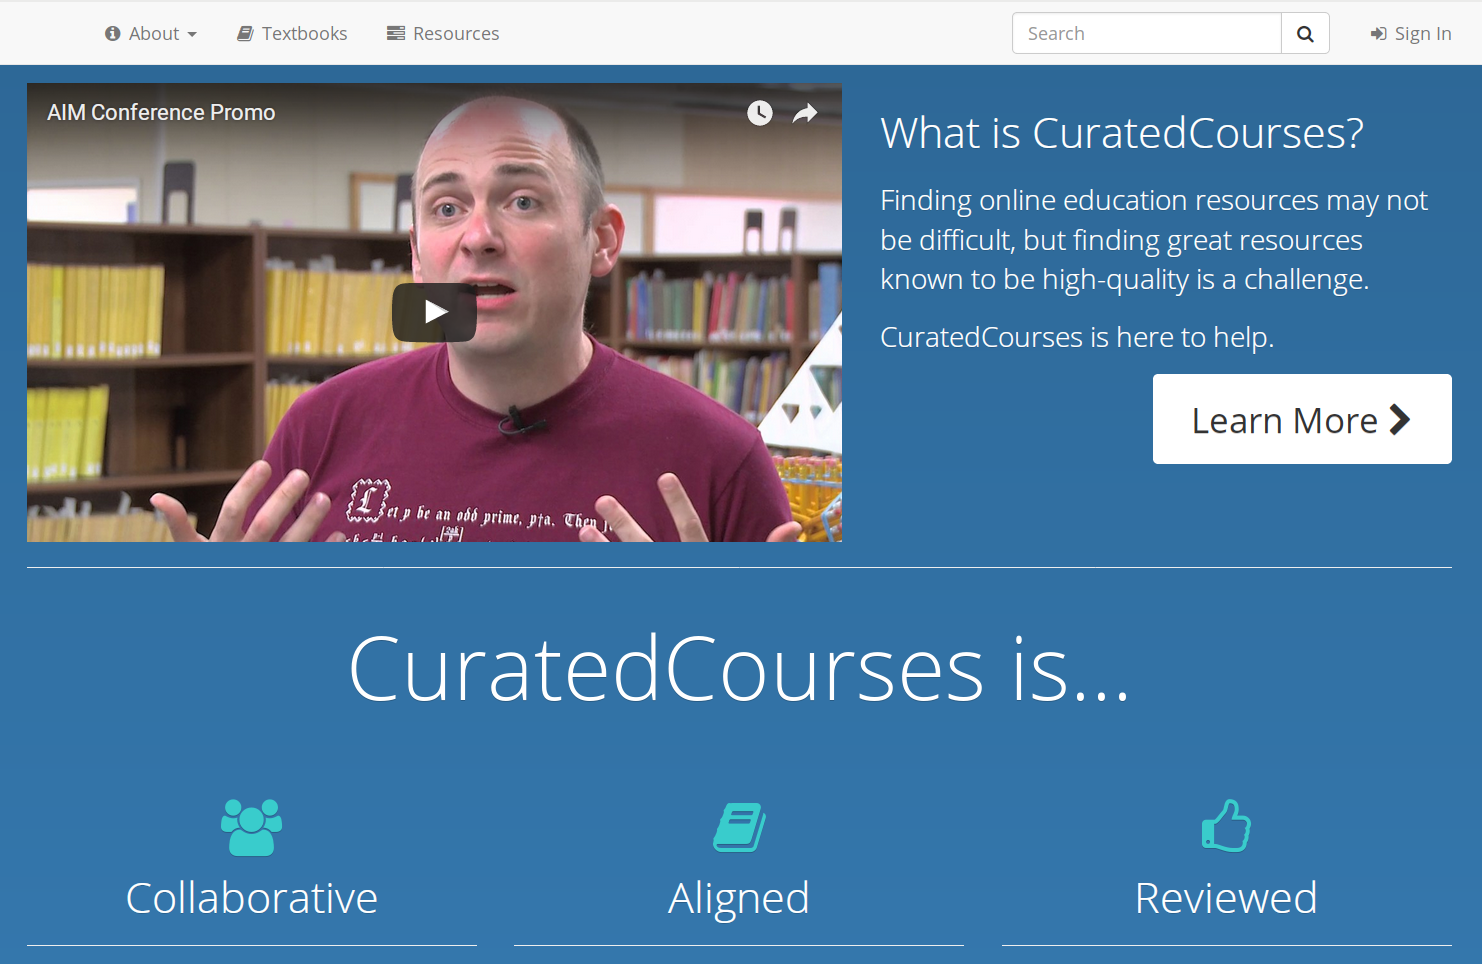
\includegraphics[width=0.52\textwidth]{landing-page.png}
  \end{wrapfigure}

  The project team developed a platform for disseminating and hosting 
  open mathematics content.

  \vspace{1ex}A resource submitted to the platform enters a moderation queue,
  permitting curation by experts, and is tagged with
  \textbf{standardized topics} and \textbf{learning outcomes},
  permitting alignment of high-quality resources to textbooks.
\end{sectionblock}